\paragraph[QuizziPedia::Front-End::Controllers\\::StringsSortingQuestionsController]{QuizziPedia::Front-End::Controllers::StringsSortingQuestionsController}
\begin{figure} [ht]
	\centering
	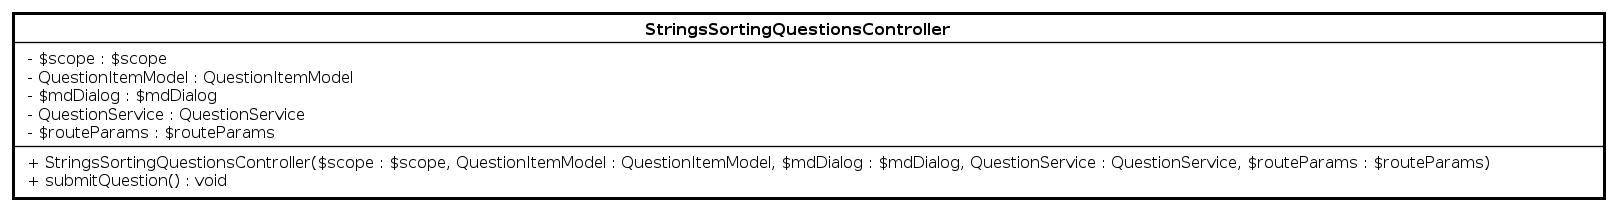
\includegraphics[scale=0.3]{UML/Classi/Front-End/QuizziPedia_Front-end_Controller_StringSortingQuestionsController.png}
	\caption{QuizziPedia::Front-End::Controllers::StringsSortingQuestionsController}
\end{figure} \FloatBarrier
\begin{itemize}
	\item \textbf{Descrizione}: questa classe permette di gestire la creazione e la modifica di una domanda a ordinamento di stringhe;
	\item \textbf{Utilizzo}: fornisce le funzionalità per inserire una nuova domanda a ordinamento di stringhe nel database e per modificarne una esistente;
	\item \textbf{Relazione con altre classi}:
	\begin{itemize}
		\item \textbf{IN \texttt{StringsSortingQuestionsModelView}}: classe di tipo \textit{modelview \ped{G}} la cui istanziazione è contenuta all'interno della variabile di ambiente \$scope di \textit{Angular\ped{G}}. All'interno di essa sono presenti le variabili e i metodi necessari per il \textit{Two-Way Data-Binding\ped{G}} tra la \textit{view\ped{G}} \texttt{StringsSortingQuestionsView} e il \textit{controller\ped{G}} \texttt{StringsSortingQuestio-\\nsController};
		\item \textbf{IN \texttt{QuestionService}}: questa classe permette di:
		\begin{itemize}
			\item Ottenere una domanda attraverso il metodo dedicato;
			\item Caricare una domanda modificata;
			\item Caricare una nuova domanda.
		\end{itemize}
		\item \textbf{IN \texttt{QuestionItemModel}}: questa classe rappresenta il modello di una domanda.
	\end{itemize}
	\item \textbf{Attributi}:
	\begin{itemize}
		\item \texttt{-} \texttt{\$scope: \$scope} \\
		Campo dati contenente un riferimento all'oggetto \$scope creato da \textit{Angular\ped{G}}, viene utilizzato come mezzo di comunicazione tra il \textit{controller\ped{G}} e la \textit{view\ped{G}}. Contiene gli oggetti che definiscono il \textit{model\ped{G}} dell'applicazione;
		\item \texttt{-} \texttt{QuestionItemModel: QuestionItemModel} \\
		Campo dati che si riferisce alla classe che rappresenta il modello della domanda;
		\item \texttt{-} \texttt{\$mdDialog: \$mdDialog} \\
		Campo dati contenente un riferimento al servizio della libreria \textit{Material for Angular\ped{G}} che permette di creare delle componenti a pop-up;
		\item \texttt{-} \texttt{QuestionService: QuestionService}: \\
		Campo dati contenente un riferimento al servizio che si occupa della gestione delle informazioni legate alle domande;
		\item \texttt{\$routeParams: \$routeParams} \\
		Campo dati contenente il riferimento all'oggetto globale \$routeParams creato da \textit{Angular\ped{G}}. Tale servizio permette di recuperare il set di variabili presenti nell'URL. 
	\end{itemize}
	\item \textbf{Metodi}:
	\begin{itemize}
		\item \texttt{+} \texttt{StringsSortingQuestionsController(\$scope: \$scope, QuestionItemModel:\\ QuestionItemModel, \$mdDialog: \$mdDialog, QuestionService: QuestionSe-\\rvice, \$routeParams: \$routeParams)} \\ 
		Metodo costruttore della classe. Se in \$routeParams sarà presente il codice univoco che rappresenta una domanda e di questa il creatore è l'utente autenticato, allora verrà scaricato attraverso il \texttt{QuestionService} il contenuto della domanda così da poterlo modificare. In caso contrario verrà mostrato un errore attraverso \$mdDialog indicando che i privilegi per tale operazione sono negati. Nel caso in cui non ci sarà tale parametro in \$routeParams verrà caricata la \textit{view\ped{G}} vuota così da poter creare una nuova domanda. \\
		\textbf{Parametri}:
		\begin{itemize}
			\item \texttt{\$scope: \$scope} \\
			Parametro contenente un riferimento all'oggetto \$scope creato da \textit{Angular\ped{G}}. Viene utilizzato come mezzo di comunicazione tra il \textit{controller\ped{G}} e la \textit{view\ped{G}}. Contiene gli oggetti che definiscono il \textit{viewmodel\ped{G}} e il \textit{model\ped{G}} dell'applicazione;
			\item \texttt{QuestionItemModel: QuestionItemModel} \\ 
			Parametro che si riferisce alla classe che rappresenta il modello della domanda;
			\item \texttt{\$mdDialog: \$mdDialog} \\
			Parametro contenente un riferimento al servizio della libreria \textit{Material for Angular\ped{G}} che permette di creare delle componenti a pop-up;
			\item \texttt{QuestionService: QuestionService}: \\
			Parametro contenente un riferimento al servizio che si occupa della gestione delle informazioni legate alle domande;
			\item \texttt{\$routeParams: \$routeParams} \\
			Parametro contenente il riferimento all'oggetto globale \$routeParams creato da \textit{Angular\ped{G}}. Tale servizio permette di recuperare il set di variabili presenti nell'URL. 
		\end{itemize}
		\item \texttt{+} \texttt{submitQuestion(): void}\\ 
		Metodo che gestisce l'evento click sul pulsante di conferma sulla domanda. Raccoglie i dati dal \textit{modelview\ped{G}} e li manda al \textit{server\ped{G}} attraverso \texttt{QuestionService}. Poi verrà effettuato il redirect alla pagina di gestione delle domande oppure al questionario che si stava creando. 
	\end{itemize}
\end{itemize}

